\section{Objective}
To study the magnetic hysteresis loop for a  massive iron core.

\section{Theory}
\subsection*{Magnetism in matter}

The magnetic state of a material can be described by a vector $\vec{M}$
called magnetization, or dipolar magnetic moment per unit volume. In vacuum, the magnetic
induction $\vec{B}$ and the applied magnetic field intensity, $\vec{H}$, are connected by the equation:
\begin{align}
    \vec{B} = \mu_o\vec{H}
\end{align}

where $\mu_o = 4\pi \cross 10-7$ Hm$^{-1}$, is the absolute magnetic permeability of vacuum. However, in a matter, magnetic induction depends on magnetization $\vec{M}$ in the following way,
\begin{align}
    \vec{B} = \mu_o(\vec{H} + \vec{M})
\end{align}

There is another important parameter called the magnetic susceptibility, $\chi$, which is a
measure of the quality of the magnetic material and defined as the magnetization produced
per unit applied magnetic field, i.e.,
\begin{align}
    \chi = M/H
\end{align}

Magnetism in solids is Broadly classified into 3 categories: diamagnetism, paramagnetism and ferromagnetism.

\begin{enumerate}
    \item \textbf{Diamagnetism} is a very weak effect observed in solids having no permanent magnetic moments. It arises due to changes in the atomic orbital states induced by the applied magnetic field. It exists in all materials but usually suppressed by other stronger effects such as para- or ferromagnetism. For diamagnetic materials, magnetization $\vec{M}$ varies linearly with $\vec{H}$ in opposite direction. Hence $\chi < 0$. Diamagnetism is temperature independent.\\
    \item \textbf{Paramagnetism} is also a weak effect, but unlike diamagnetism, the magnetic moment is aligned along the direction of applied magnetic field. Certain atoms and ions (oxygen, air, iron salts, etc.) have a permanent magnetic moment of their own. Without applied magnetic field, these are oriented randomly. Therefore they don’t show any magnetization on a macroscopic scale. On applying an external magnetic field, a non-zero macroscopic magnetic moment $\vec{M}$ arises since all the magnetic momenta are aligned along the applied field. The magnetization $\vec{M}$ initially varies linearly with $\vec{H}$ and then saturates at a value Ms, called saturation magnetization. This saturation condition corresponds to the complete alignment of the magnetic dipoles along the applied field direction. However, once the applied field is removed, thermal agitation in the material is enough to disorient the atoms. Paramagnetic materials have a small, positive $\chi$. Paramgnetism is temperature dependent.\\
    \item \textbf{Ferromagnetism} is associated with the presence of permanent magnetic dipoles where the magnetic momenta of adjacent atoms are aligned in a particular direction, even in the absence of an external magnetic field. This is known as spontaneous magnetization. A ferromagnetic material contains a number of small regions called domains, which are having spontaneous magnetization values of different magnitude. On application of an external magnetic field $\vec{H}$, these domains align in the direction of $\vec{H}$ and develop a strong macroscopic magnetization $\vec{M}$. The value of $\chi$ for a ferromagnetic material is large and positive. Ferromagnetism is temperature dependent as it exists below a certain temperature known as Curie temperature $T_C$. Some examples of ferromagnetic materials are iron, cobalt and nickel.
\end{enumerate}

\subsection*{Hysteresis}
Hysteresis loop (Fig. \ref{fig:1}) shows the relation between the magnetization $\vec{M}$ or the magnetic induction $\vec{B}$ as a function of $\vec{H}$. It is a characteristic property of any ferromagnetic material. The dotted line in Fig. 1 shows that as the applied field is increased the magnetization in the domains grows along the so-called easy direction of magnetization and finally attains a \textbf{saturation value} at $B_S$. At this point all the domains point along the direction of applied magnetic field. On decreasing the field, $\vec{B}$ is not reversible and possesses a non-zero value called \textbf{remanent induction}, $B_r$. It can be reduced to zero by applying a reverse magnetic field known as coercive magnetic field or \textbf{coercivity}, $H_C$. A similar variation is observed as the reverse field is varied resulting in a closed loop known as hysteresis loop.


\begin{figure}[H]
    \centering
    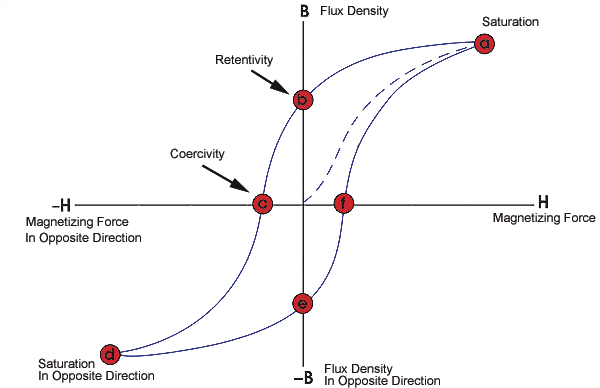
\includegraphics[width=1\columnwidth]{images/f1.png}
    \caption{Hysteresis Loop}
    \label{fig:1}
\end{figure}

\subsection*{Degaussing}
Degaussing is the process of decreasing or eliminating a remnant magnetic field present in a ferromagnetic material due to hysteresis. Annealing, hammering or applying a rapidly oscillating magnetic field (Fig. \ref{fig:2}) are some of the methods of degaussing which tend to release the domain walls from their pinned state, and the domain boundaries tend to move back to a lower energy configuration. 

\begin{figure}[H]
    \centering
    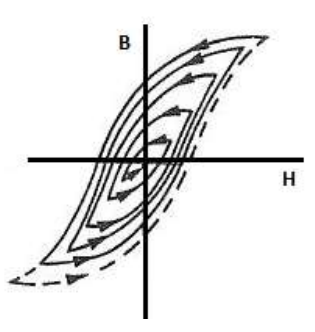
\includegraphics[width=0.6\columnwidth]{images/f2.png}
    \caption{Degaussing Curve}
    \label{fig:2}
\end{figure}

\section{Experimental Setup}

\subsection*{Apparatus}
\begin{enumerate}
    \item Iron core
    \item Pair of coils (600 turns each, current limit 2A)
    \item DC power supply
    \item Digital gauss meter (DGM) with hall probe
    \item Reversible switch
    \item Connecting wires
\end{enumerate}